\documentclass[main.tex]{subfiles}

\begin{document}
\chapter{Computational Details\label{ch:computation}}
%\epigraph{It's a secret to everybody.}{a Moblin in \textit{The Legend of Zelda}}

\section{Parallel computing\label{sec:parallel_computing}}

The following section will give an overview of the technical aspects of running computer code (such as \QE) on massively parallel computing environments (such as the PHYSnet compute cluster).
The information presented in this section comes from the textbook on high-performance computing by Hager and Wellein \cite{hager_introduction_2010}.

\subsection{On scalabilty}\label{sub:scalability_general}

In scientific computing, one can identify two distinct reasons for distributing workloads to multiple processors:
\begin{itemize}
    \item The execution time on a single core is not sufficient. The definition of sufficient is dependent on the specific task and can range from \enquote{over lunch} to \enquote{multiple weeks}.
    \item The memory requirements grow outside the capabilities of a single core.
\end{itemize}

In order to judge how well a task can be parallelized, usually a scalability metric is employed, for example:
\begin{itemize}
    \item How fast can a problem be solved with \(N\) processors instead of one?
    \item What kind of bigger problem (finer resolution, more particles, etc.) can be solved with \(N\) processors?
    \item How efficiently are the resources utilized?
\end{itemize}
In this thesis, the main concern is speeding up the execution of extensively expensive calculations with a fixed problem size, so the first metric will be used to judge the quality of parallelization.
This metric is called speedup and is defined as 
\begin{equation}\label{eq:definition_speedup}
    S = \frac{T_1}{T_N}\,, 
\end{equation}
where \(T_1\) is the execution time on a single processor and \(T_N\) is the execution time on \(N\) processors.
In the ideal case, where all the work can be perfectly distributed among the processors, all processors need the same time for their respective workloads and don't depend on others processors finishing their workload to continue, the execution time on \(N\) processors would be \(\frac{T_1}{N}\), so inserting this into eq. \ref{eq:definition_speedup} gives a speedup of
\begin{equation}
    S = \frac{T_1}{\frac{T_1}{N}} = N\,.
\end{equation}

In reality, there are many factors either limiting or in some cases supporting parallel code scalability. Limiting factors include:
\begin{itemize}
    \item \emph{Algorithmic limitations}: when parts of a calculation are mutually dependent on each other, the calculation cannot be fully parallelized
    \item \emph{Bottlenecks}: in any computer system exist resources which are shared between processor cores with limitations on parallel access. This serializes the execution by requiring cores to wait for others to complete the task which uses the shared resources in question
    \item \emph{Startup Overhead}: introducing parallelization into a programm necessarily introduces an overhead, e.g. for distributing data across all the processors
    \item \emph{Communication}: often solving a problem requires communication between different cores (e.g. exchange of interim results after a step of the calculation). Communication can be implemented very effectively, but can still introduce a big prize in computation time
\end{itemize}
On the other hand, \emph{better caching} can lead to better scaling than \(S = N\): as optimal performance per core is achieved when all the data can be kept in cache, reducing the data size per processor by distributing data among more processors can lead to each individual processor being faster than in the single core case.

A simple ansatz for modeling speedup with these limitations in mind was first derived by Gene Amdahl \cite{amdahl_validity_1967}.
Assuming the work that needs to be done is split into a part which cannot be parallelized \(s\) and a part which can be parallelized ideally \(p\), serial time can be normalized to 1:
\begin{equation}
    T_1 = s + p = 1
\end{equation}
The time for solving the problem on \(N\) processors is then
\begin{equation}
    T_N = s + \frac{p}{N}\,.
\end{equation}
The speedup is now
\begin{equation}\label{eq:amdahls_law}
    S = \frac{T_s}{T_p} = \frac{1}{s + \frac{p}{N}} = \frac{1}{s + \frac{1 - s}{N}}
\end{equation}
This equation is called \emph{Amdahl's law} and is plotted in fig. \ref{fig:amdahl} over a range of processors for a few different values of \(s\).

\begin{figure}[ht!]
    \centering
    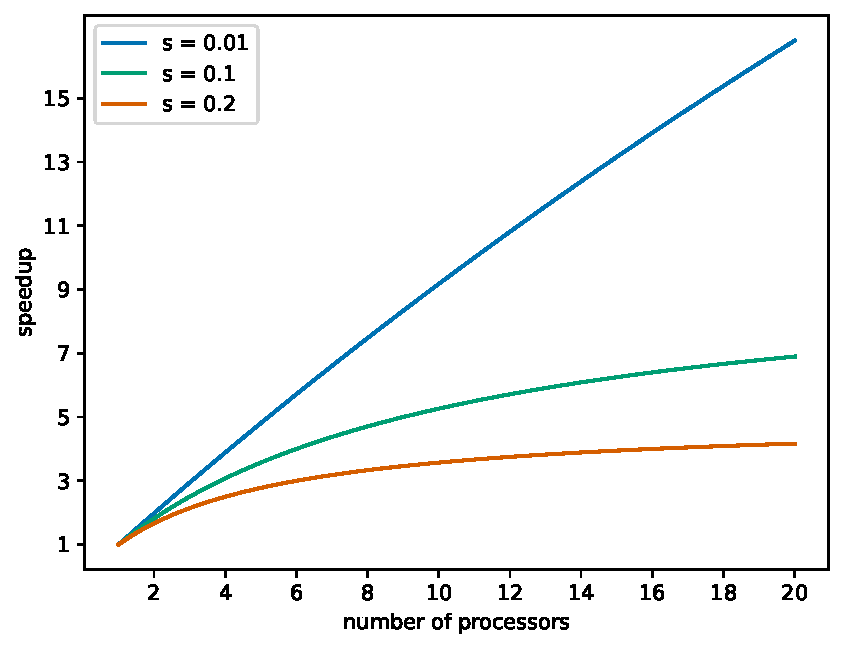
\includegraphics[width=0.6\textwidth]{amdahl.pdf}
    \label{fig:amdahl}
    \caption{Amdahl's law for different portions of not parallelizable workload \(s\)}
\end{figure}

\subsection{Evaluating the scalability of \QE calculations}\label{sub:scalability_qe}

In the \QE output, a time report listing is printed at the end.
This time report includes \gls{cpu_time} and \gls{wall_time}, from those three different metrics of scalability can be calculated:
\begin{itemize}
    \item runtime: absolute runtime (\gls{wall_time}) of the compute job
    \item speedup: runtime on \(N\) processors divided by runtime on a single core
    \item \gls{wait_time}: percentage of \gls{wall_time} not used by \QE process, so writing to disk, waiting for IO devices or other processes, etc. (calculated as (\gls{wall_time} - \gls{cpu_time}) / \gls{wall_time})
\end{itemize}
For analysis mainly speedup will be used to evaluate the scalability of \QE calculation.
It makes comparing the scaling of calculations with different absolute runtimes easy: as discussed in sec. \ref{sub:scalability_general}, optimal scaling is achieved when the speedup has a slope of one, independent of the runtime.

Regardless, the other two parameters should also always be considered: in the end, absolute runtime is the most important factor and should govern the decision of how much resources are used for solving a particular problem.
For instance, a problem with a single core runtime of \(\SI{600}{\s}\), a speedup of 100 would mean a runtime of \(\SI{6}{\s}\), whereas a speedup of 200 would mean a runtime of \(\SI{3}{\s}\).
Even with optimal scaling, the 100 processors needed for the speedup of 200 could be considered wasted for just \(\SI{3}{s}\) of saved time.
On the other hand, for a problem with a single core runtime of \(\SI{2400}{\hour}\), the difference between a speedup of 100 (runtime \(\SI{24}{\hour}\)) and 200 (runtime \(\SI{12}{\hour}\)) is the difference between needing to wait a whole day for the calculation and being able to let the job run overnight and continue working in the morning, so using 100 more processors for that can be considered a good use of resources.

As for the \gls{wait_time}, this metric can be used to separate the different factors of poor parallelization discussed in \ref{sub:scalability_general}.
Startup overhead is easy to identify, as this should be a small, near constant percentage of the absolute runtime.
This of course can vary depending on how complex data distribution is, but there should at least not be a strong dependence on the number of processors, as only a small amount of communication is needed.
Communication and bottlenecks on the other hand both introduce wait time which depends on the number of processors.
Differentiating between them is relies on knowledge of the specific hardware of the system running the calculations, so how many cores are on a single chip, motherboard or node, which resources are shared between how many cores, etc.\,.

For this interpretation to be meaningful, the CPU and wall times reported by \QE have to be accurate, because they are trusted without verification.
Just as an example for the pitfalls of this approach, when executing programs on multiple processors in parallel, \gls{cpu_time} is measured per processor, so some kind of truncation is done when a single number (such as in \QE) is reported.
Whether this is taking the average over all processors, just reporting the time for a single processor or any other kind of truncation is unclear.

However, the notion of using the difference between \gls{wall_time} and \gls{cpu_time} for evaluating the quality of parallelization is supported by the user guide for one of the \QE modules \cite{noauthor_pwscf_nodate} (sec. 4.5), therefore it will also be used as a qualitative measure of good parallelization in this thesis.

\section{\QE}\label{sec:qe}

\QE (opEn-Source Package for Research in Electronic Structure, Simulation, and Optimization) \cite{giannozzi_quantum_2009,giannozzi_advanced_2017} is a collection of packages implementing (among others) the techniques described in sec. \ref{sec:theory_dft} and \ref{seq:theory_dfpt} to calculate electronic structure properties (module \texttt{PWscf}) as well as phonon frequencies and eigenmodes (module \texttt{PHonon}).

\subsection{Compilation of \QE}\label{sub:qe_compilation}

As the core of this thesis is an in depth examination of the \QE software and ways its performance can be optimized, a discussion of the way it is compiled is needed.
The information in this section is taken from the \QE 7.0 user guide \cite{noauthor_quantum_nodate}.

The \QE distribution is packaged with everything needed for simple, non-parallel execution, the only additional software needed are a minimal Unix environment (a shell like \texttt{bash} or \texttt{sh} as well as the utilities \texttt{make} \texttt{awk} and \texttt{sed}) and a Fortran compiler compliant with the F2008 standard.
For parallel execution, also \gls{mpi} libraries and an \gls{mpi} aware compiler need to be provided.

\QE needs three external mathematical libraries, \gls{blas} and \gls{lapack} for linear algebra as well as an implementation of \gls{fft} for fourier transforms.
In order to make the installation as easy as possible, \QE comes with a publicly available reference implementation of the \gls{blas} routines, the publicly available \gls{lapack} package and an older version of FFTW (Fastest Fourier Transform in the West, an open source implementation of \gls{fft}).
Even though these libraries are already optimized in terms of the algorithms implemented, usage of libraries implementing the same routines which can use more specific CPU optimizations significantly improves performance (e.g. libraries provided by Intel can use CPU optimizations not present on AMD processors).

On the PHYSnet cluster, a variety of software packages are available as modules.
The benchmarks in this thesis were made using the following module combinations:
\begin{itemize}
    \item \texttt{openmpi/4.1.1.gcc10.2-infiniband}: \gls{openmpi} 4.1.0 (implies usage of \QE provided \gls{blas}/\gls{lapack})
    \item \texttt{openmpi/4.1.1.gcc10.2-infiniband openblas/0.3.20}: \gls{openmpi} 4.1.0 and \gls{openblas} 0.3.20
    \item \texttt{scalapack/2.2.0}: \gls{openmpi} 4.1.0, \gls{openblas} 0.3.20 and \gls{scalapack} 2.2.0
    \item \texttt{intel/oneAPI-2021.4}: \gls{oneapi} 2021.4
\end{itemize}

\QE offers a configuration script to automatically find all required libraries.
As the default options of the \texttt{configure} script work well in the use case of this thesis, all compilations were made using the minimal commands
\begin{verbatim}
    module load <module names>
    ./configure --with-scalapack=no|yes|intel
\end{verbatim}
with the scalapack options yes (when using \texttt{scalapack/2.2.0}), intel (when using \\ \texttt{intel/oneAPI-2021.4}) and no otherwise.

The output of the configuration script gives information about the detected libraries.
In the following output, the Intel \gls{oneapi} package was loaded, so \gls{blas} and \gls{scalapack} libraries from that package will be used, whereas the included \gls{fft} library will be used:
\begin{verbatim}
    The following libraries have been found:
    BLAS_LIBS=  -lmkl_intel_lp64  -lmkl_sequential -lmkl_core
    LAPACK_LIBS=
    SCALAPACK_LIBS=-lmkl_scalapack_lp64 -lmkl_blacs_intelmpi_lp64
    FFT_LIBS= 
\end{verbatim}

\subsection{Parallelization capabilities implemented in \QE}\label{sub:qe_parallelization}

\QE is intended to be used in parallel environments and as such offers possibilities to manage how the work is parallelized.
This section introduces the parallelization capabilities of the \texttt{PWscf} and \texttt{PHonon} modules and explores how they potentially affect the scaling behavior of \QE. The information in this section stems from the user guides for the two modules \cite{noauthor_pwscf_nodate, noauthor_phonon_nodate}

\begin{figure}[htb!]
\label{fig:diagram-scf-calculations}
%\centering
\begin{tikzpicture}[
    squarednode/.style={rectangle, draw=purple!60, fill=purple!5, thick, minimum size=5mm, text centered, text width=8cm,},
    node distance=0.5cm]
    \tikzset{every node/.style={inner sep=8pt}}
    %Nodes
    \node[squarednode]      (init)          {initial \(n(\vb*{r})\)};
    \node[squarednode]      (step_1)    [below= of init]  {calculate \(v_H [n(\vb*{r})]\) and \(v_{XC} [n(\vb*{r})]\)};
    \node[squarednode]      (step_2)    [below= of step_1]      {fourier transform potentials};
    \node[squarednode]      (step_3)    [below= of step_2]      {solve \acrshort{kohn_sham} equations in reciprocal space};
    \node[squarednode]      (step_4)    [below= of step_3]      {fourier transform wavefunctions};
    \node[squarednode]      (step_5)    [below= of step_4]      {calculate \(n(\vb*{r})\) and \(E [n(\vb*{r})]\)};
    \node[squarednode]      (done)      [below= of step_5]      {done if change in \(E\) is small enough};
    
    %Lines
    \draw[->] (init.south) -- (step_1.north);
    \draw[->] (step_1.south) -- (step_2.north);
    \draw[->] (step_2.south) -- (step_3.north);
    \draw[->] (step_3.south) -- (step_4.north);
    \draw[->] (step_4.south) -- (step_5.north);
    \draw[->] (step_5.east) to [out=30,in=-30] (step_1.east);
    \draw[->] (step_5.south) -- (done.north);
\end{tikzpicture}
\caption{Flowchart of an algorithm to iteratively solve the \acrshort{kohn_sham} equations with the use of fourier transform}
\end{figure}
Fig. \ref{fig:diagram-scf-calculations} shows a possible approach to solving the \acrshort{kohn_sham} equations.
A few possibilities for parallelization of calculations can be derived from that.

First of all, the real/reciprocal are discretized to allow for numerical treatment, these grids can be distributed among processors, meaning the orbitals in the plane wave basis set as well as charges and densities.
This distribution of data mainly works around memory constraints, as using more processors lowers the memory requirement for every single processor.
Going further, \QE automatically parallelizes all linear algebra operations on this real space/reciprocal grid.
The price to pay for this parallelization is the need for communication between processors: as an example, fourier transforms always need to collect and distribute contributions from and to the whole reciprocal/real grid in order to transform between them.
This kind of parallelization is called \emph{PW (plane wave)} or \emph{R\&G (real \& reciprocal)} parallelization. 

As discussed in sec. \ref{sub:theory_basis_set}, the density in the plane wave basis set is a sum over different k points, where the calculation for these are independent of each other until calculating the density \(n( \vb*{r})\).
In \QE this is implemented such that a separation of the total number of processors into smaller pools, each doing the calculations for a set of k points is possible.
This is called \emph{k point parallelization}.
The CLI parameter \texttt{-nk <number of pools>} determines how many pools the total number of processor \(N\) is split into.
Hence, the resulting number of processors in one pool is \(\nicefrac{N}{N_k}\).
Within one k point processor pool, the PW parallelization with its heavy communication is automatically applied.

In a level of parallelization independent of that, \QE can use \gls{scalapack} to parallelize (among other things) the iterative orthonormalization of \acrshort{kohn_sham} states.
This parallelization level is called \emph{linear algebra parallelization} and is controlled by the CLI parameter \texttt{-nd <number of processors in linear algebra group>}.
Importantly, this parameter sets the size for the linear algebra group in every k point processor pool, so the number of processors in the linear algebra group has to be smaller than the number of processors in one pool.
Furthermore, the arrays on which the calculations are performed on are distributed in a 2D grid among processors, so the number of processors in the linear algebra group has to be a square number.

In the case of the \texttt{PHonon} module, the representation of states in a plane-wave basis set stays the same, so all three parallelization schemes mentioned for the \texttt{PWscf} module can also be employed.
Furthermore, as calculations for two phonon wave vectors \(\vb*{q}, \vb*{q}^{\prime}\) are not coupled (as different wave vectors lead to different perturbations and as such independent self-consistent equations), they can be split up into images.
The concept of image parallelization in \QE is actually more general than just for phonon calculations, as other kinds of independent iterative calculations can also be run with image parallelization.
The parameter controlling image parallelization is \texttt{ni <number of images>}.
Following this, the number of processors in one k point pool is then given by \(N / N_i / N_k\).

\section{Hardware configuration of the PHYSnet cluster}\label{sec:hardware_physnet}

All calculations were run on a reserved subset of the \texttt{infinix} queue on the PHYSnet compute cluster, with 20 nodes.
As of time of writing, the nodes in this queue are equipped with two Intel Xeon E5-2680 CPUs, as such providing 20 cores per node, 10 per chip and 200 processors in the whole queue.

\todo{speed comparison, why is this important?}

%Knowing the specific hardware configuration the calculations are run on is important, as that provides a scale of different communication speeds:
%\begin{itemize}
%    \item between processors on one chip:
%    \item between processors on one motherboard:
%    \item between processors on different nodes:
%\end{itemize}
%\todo{speed comparison between processors on one chip, on one motherboard, between nodes (infiniband)}
%This gives guidelines on how well calculations can be parallelized on different numbers of processors.
%As an example, any calculation with a massive need for communication, for example the calculations one the PW 

\end{document}
